\documentclass[border=4pt]{standalone}
\usepackage{tikz}\usetikzlibrary{positioning,arrows.meta}
\usepackage{siunitx}
\begin{document}
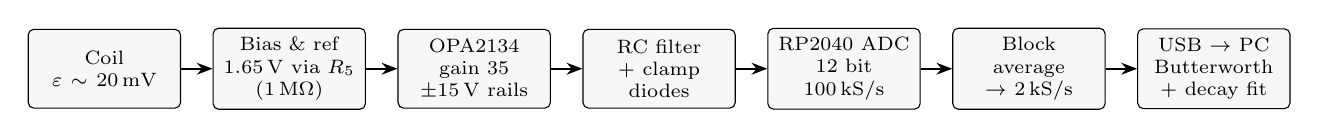
\begin{tikzpicture}[font=\scriptsize,node distance=4mm,
  b/.style={draw,rounded corners=2pt,align=center,minimum height=10mm,text width=17mm,fill=gray!6},
  a/.style={-{Stealth[length=2mm]},thick}]
\node[b] (coil) {Coil\\$\varepsilon\sim\SI{20}{mV}$};
\node[b,right=of coil] (bias) {Bias \& ref\\$\SI{1.65}{V}$ via $R_5$\\(\SI{1}{M\ohm})};
\node[b,right=of bias] (amp) {OPA2134\\gain 35\\$\pm\SI{15}{V}$ rails};
\node[b,right=of amp] (prot) {RC filter\\+ clamp\\diodes};
\node[b,right=of prot] (adc) {RP2040 ADC\\12 bit\\\SI{100}{kS/s}};
\node[b,right=of adc] (dec) {Block\\average\\$\to$ \SI{2}{kS/s}};
\node[b,right=of dec] (pc) {USB $\to$ PC\\Butterworth\\+ decay fit};
\foreach \x/\y in {coil/bias,bias/amp,amp/prot,prot/adc,adc/dec,dec/pc} \draw[a] (\x)--(\y);
\end{tikzpicture}
\end{document}
